\section{Purpose and objectives of the study} \label{purpose}

In this thesis I set out to research the usability of force feedback in the context of \glspl{dmi}. I wanted to find out how the user experience differs in \glspl{dmi} with and without force feedback, especially whether users would find inclusion of force feedback helpful and enjoyable. Sometimes using something new can feel difficult or unpleasant, while in reality it is actually helping the user to reach their goal. That is why in comparison to the subjective experience of the users, I also wanted to see if force feedback could provide any objective, measurable benefit. My research questions are:

\begin{enumerate}
	\item How do users find the helpfulness and enjoyability of using a \gls{dmi} with force feedback compared to one without it?
	\item Does inclusion of force feedback provide measurable benefit in using a \gls{dmi}?
\end{enumerate}

Thus, I needed both qualitative and quantitative data for the research, which I collected conducting user studies. I gave the users tasks using a \gls{dmi} with various kinds of force feedback and no force feedback, surveyed their subjective experience with \gls{nasa-tlx} load questionnaire and interviews, and measured objective performance by measuring time and accuracy to finish the tasks. User study structure is explained in more detail in Chapter \ref{userstudy}.

\section{Design and implementation}

To test usability of force feedback on a \gls{dmi}, I designed and built a simple analogue modeling synthesizer with a motorized slider called HapSynth, where the motor is used to provide force feedback by moving the slider in ways which apply pressure to the user's fingers. There were at least one commercial synthesizer (\cite{melbourneinstruments2024}) and couple modular synthesizer modules (\cite{dmm2024, submatrix2024}) that had some force feedback features, but they all were expensive, hard to obtain, or didn't have the needed features for the research, hence building a custom device was appropriate. Building on top of FireFader (\cite{berdahl-kontogeorgakopoulos2013}) would have been a valid starting point, but I wanted to have the audio and force feedback generated within the device. FireFader offloads those tasks to a computer, thus I ended up not using FireFader but designing the whole system from scratch. I started my design process by setting these design goals for the device:

\begin{enumerate}
	\item The device must be electronically and mechanically simple (i.e. no \gls{smd} components).
	\item The device must have one or more input methods that can provide some force feedback to the user.
	\item The device must be as compact as possible for easy transportation between locations.
\end{enumerate}

To comply with the first requirement, I chose to make a digital synthesizer using analogue modeling synthesis technique. Analogue synthesis requires more electrical components and know-how than digital synthesis which can use just one microprocessor to generate sound. I have empirically observed subtractive synthesis/analogue modeling to be a popular form of synthesis and usually considered the easiest synthesis method to learn and understand, thus making it appropriate method for a user study where participants don't need to have any prior knowledge.

For the force feedback enabling input method I decided to use a motorized slider. I considered various other motorized components such as rotational potentiometers, rotary encoders, and piano keys such as presented in \textcite{timmermans2020}, but chose to use motorized sliders as those are readily available as easy-to-use, pre-made assemblies, unlike other options which either didn't come as pre-made assemblies, meaning they required excess amount of mechanical engineering to work, or they didn't meet specifications for the projects (i.e. motor was not powerful enough to provide any meaningful force feedback). As those motorized slider assemblies are relatively expensive and require comparatively lot of power to work, I opted to have just one to keep the cost down and power distribution simpler.

To allow just one slider to control several different sound synthesis parameters, I added an array of buttons the user can use to select which parameter they want the slider to map to. To test different force feedback modes, I also added another array of buttons to select which force feedback mode to apply to the slider. I selected to implement the six basic force feedback modes presented in \textcite{kretz2004} and 15 arbitrary synthesis parameters that I felt are quite common in analogue modeling synthesizers listed in Table \ref{parameters}.

\begin{table}[h]
	\centering
	\begin{tabularx}{\textwidth}{|c|X|}
		\hline
		\thead{Group} & \thead{Parameter} \\
		\hline
		\multirow{3}{*}{Oscillator}
			& Pitch \\\cline{2-2}
			& Pulse width modulation \\\cline{2-2}
			& LFO amount to pulse width modulation \\
		\hline
		\multirow{2}{*}{Mixer}
			& Sub oscillator volume \\\cline{2-2}
			& Noise volume \\
		\hline
		\multirow{5}{*}{Filter}
			& Cutoff frequency \\\cline{2-2}
			& Resonance \\\cline{2-2}
			& Drive \\\cline{2-2}
			& Envelope generator amount to cutoff frequency \\\cline{2-2}
			& LFO amount to cutoff frequency \\
		\hline
		\multirow{4}{*}{Envelope generator (EG)}
			& Attack time \\\cline{2-2}
			& Decay time \\\cline{2-2}
			& Sustain volume \\\cline{2-2}
			& Release time \\
		\hline
		\multirow{1}{*}{Low frequency oscillator (LFO)}
			& Frequency \\
		\hline
	\end{tabularx}
	\caption{Synthesis parameters exposed in HapSynth's user interface.}
	\label{parameters}
\end{table}

Figure \ref{sketch} shows the initial sketch for HapSynth layout. I later rotated it $180^\circ$ to allow data, power, and audio connectors to face away from the user (the size of the motorized slider assembly didn't allow the connectors to be on the same side of the device), and added a "Shift"-button to access secondary functions (reset synthesis parameters to their initial values, calibrate slider, and apply "presets", the target synthesis parameter values of each individual task). Appendix \ref{ch:button} shows the final button layout sans the "Shift"-button.

\begin{figure}[h!]
	\centering
	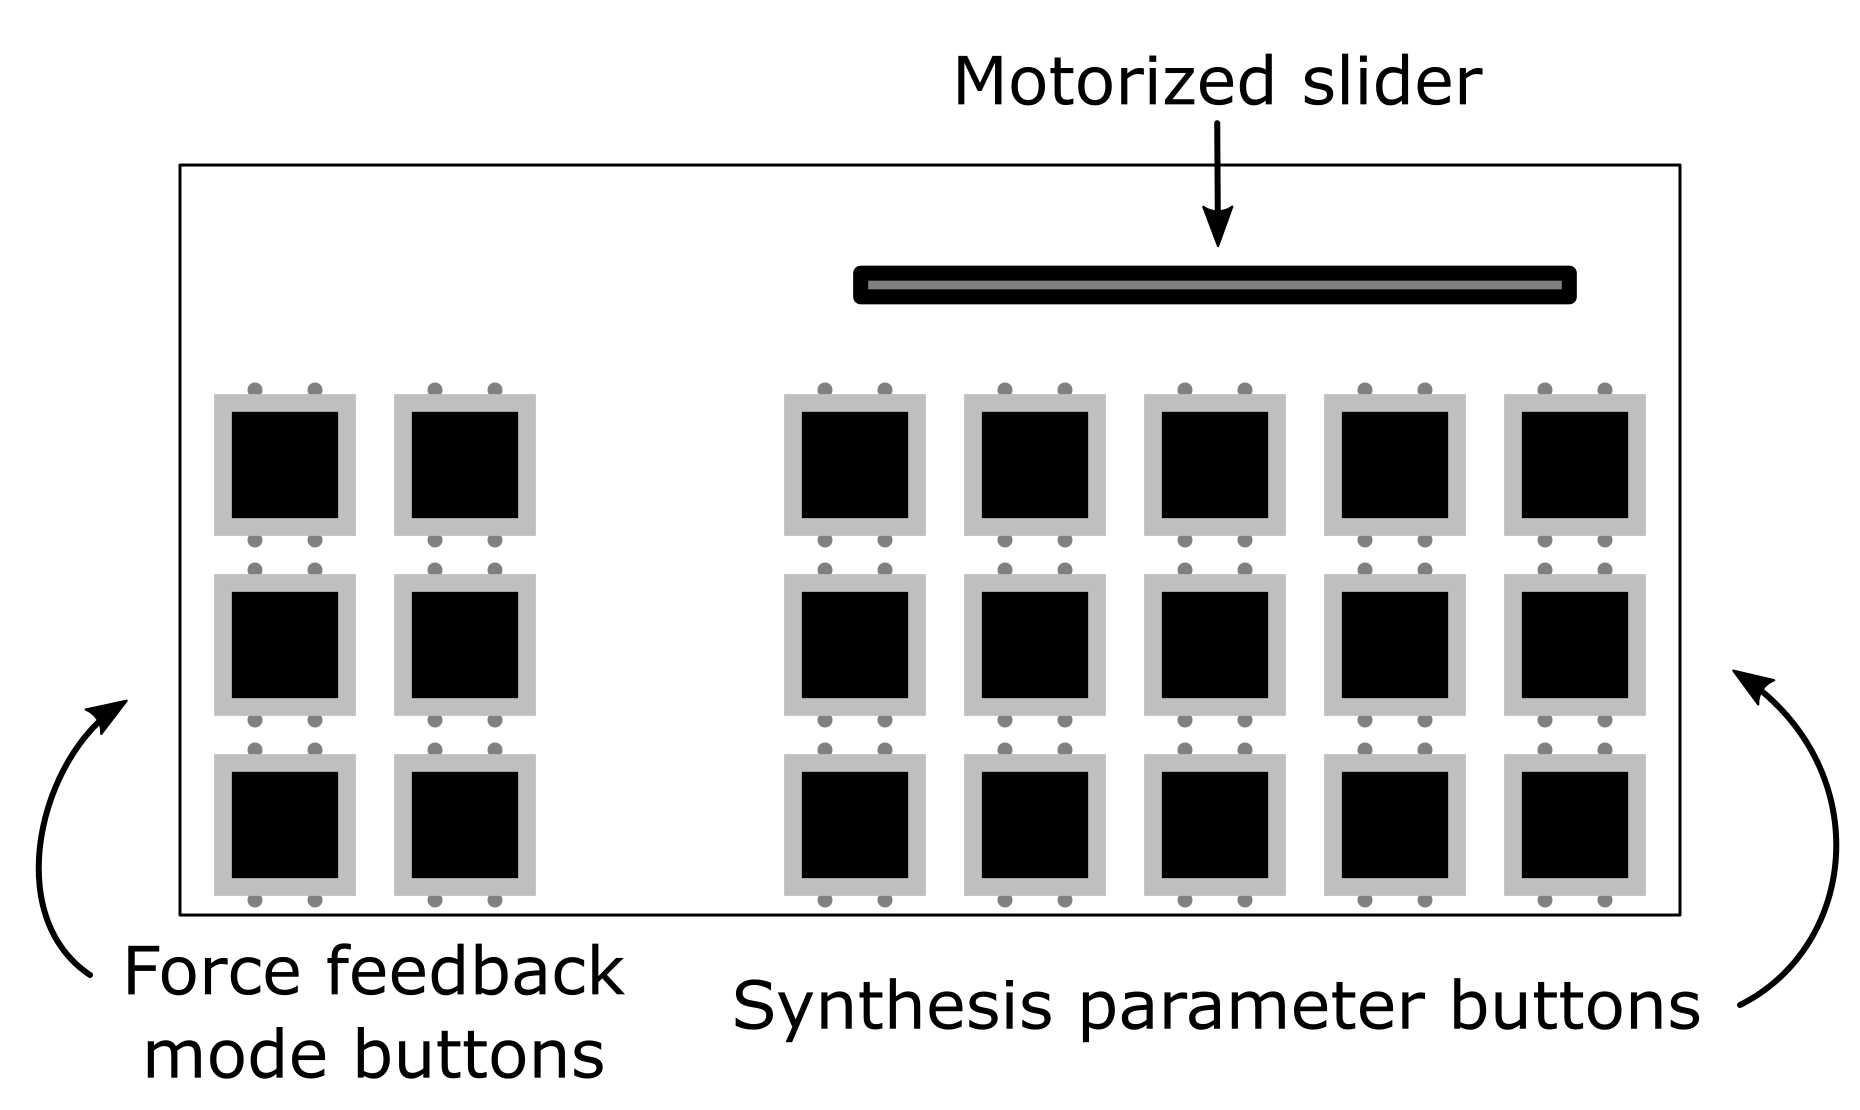
\includegraphics[width=1.0\linewidth]{figures/Adaptive.png}
	\caption{Early sketch of HapSynth.}
	\label{sketch}
\end{figure}

For processing I used Teensy 4.0 with ARM Cortex-M7 processor. Its floating-point unit, dedicated digital signal processing instructions, and Teensy Audio library (\cite{pjrc2023}) make it a good fit for audio applications. For the motorized slider I used Bourns PSM60-081A-103B2, which is mainly intended for mixing consoles (\cite{bourns2020}). For some of the force feedback modes to function properly the device needs to detect whether the slider is currently being touched or not, but implementing the capacitive touch detection directly on the Teensy took too much processing resources to be a viable option. I solved that by moving the detection to a co-processor, an Adafruit Trinket 5V microcontroller, from which the Teensy reads the current status with a simple \texttt{digitalRead} function. I soldered everything to proto boards (see Appendix \ref{ch:schematics} for schematics and Appendix \ref{ch:bom} for bill of materials) and 3D-printed a bottom case to hold the device in place while operated one handed. See Figure \ref{proto} for a photo of the finished prototype.

\begin{figure}[h]
	\centering
	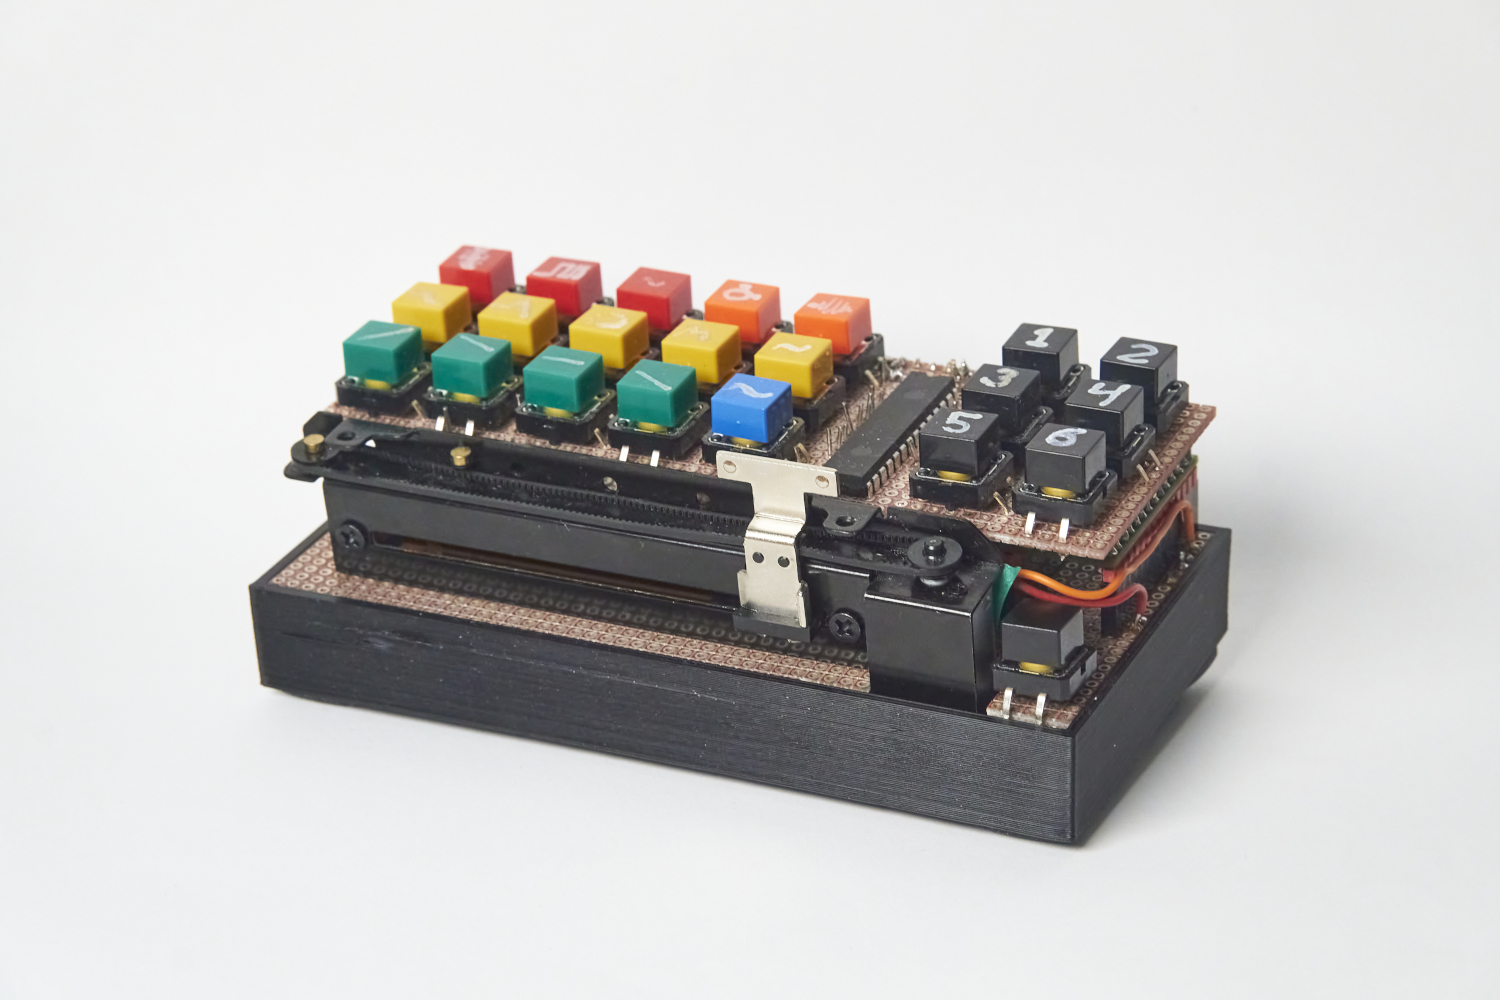
\includegraphics[width=1.0\linewidth]{figures/HapSynth.jpg}
	\caption{Finished prototype of HapSynth.}
	\label{proto}
\end{figure}

I programmed the software with Arduino programming language using aforementioned Teensy Audio library for the sound generation. The software consists of two main methods, \texttt{setup}, and \texttt{loop}. \texttt{setup}-method is run once to initialize the hardware and to set up the synthesis engine (\texttt{Synth}), while \texttt{loop}-method is executed repeatedly to read midi messages and voltages and to update \texttt{Synth}. \texttt{loop}-method updates synthesis parameter values by calling \texttt{update}-method of the currently selected synthesis parameter (\texttt{SynthParam}) and sets the direction and speed of the motor of the slider by calling \texttt{update}-method of the \texttt{SynthParam}'s force feedback mode (\texttt{HapticMode}) that matches the currently active mode. Changing active synthesis parameter and force feedback mode are handled with interrupts, which are set up in \texttt{setup}-method. See Figure \ref{classdiagram} for the class diagram. User interactions were logged through serial, printing out time since the start of the program and the name of the pressed button (either the name of the force feedback mode or the synthesis parameter selected) or a list of the values of all synthesis parameters used in the study, current force feedback mode, and current synthesis parameter whenever slider was released.

Source code for HapSynth software among other files such as the STL-file for the case are published under MIT-licence in a GitHub repository (see Appendix \ref{ch:github}). Open sourcing allows anyone to inspect the code, learn from it, and possibly provide further improvements. Functions and force feedback modes are demonstrated in a YouTube video (see Appendix \ref{ch:youtube}). Note that in the video force feedback modes are in different order than presented in this thesis, refer to the video description for additional details.

\begin{figure}[h]
	\centering
	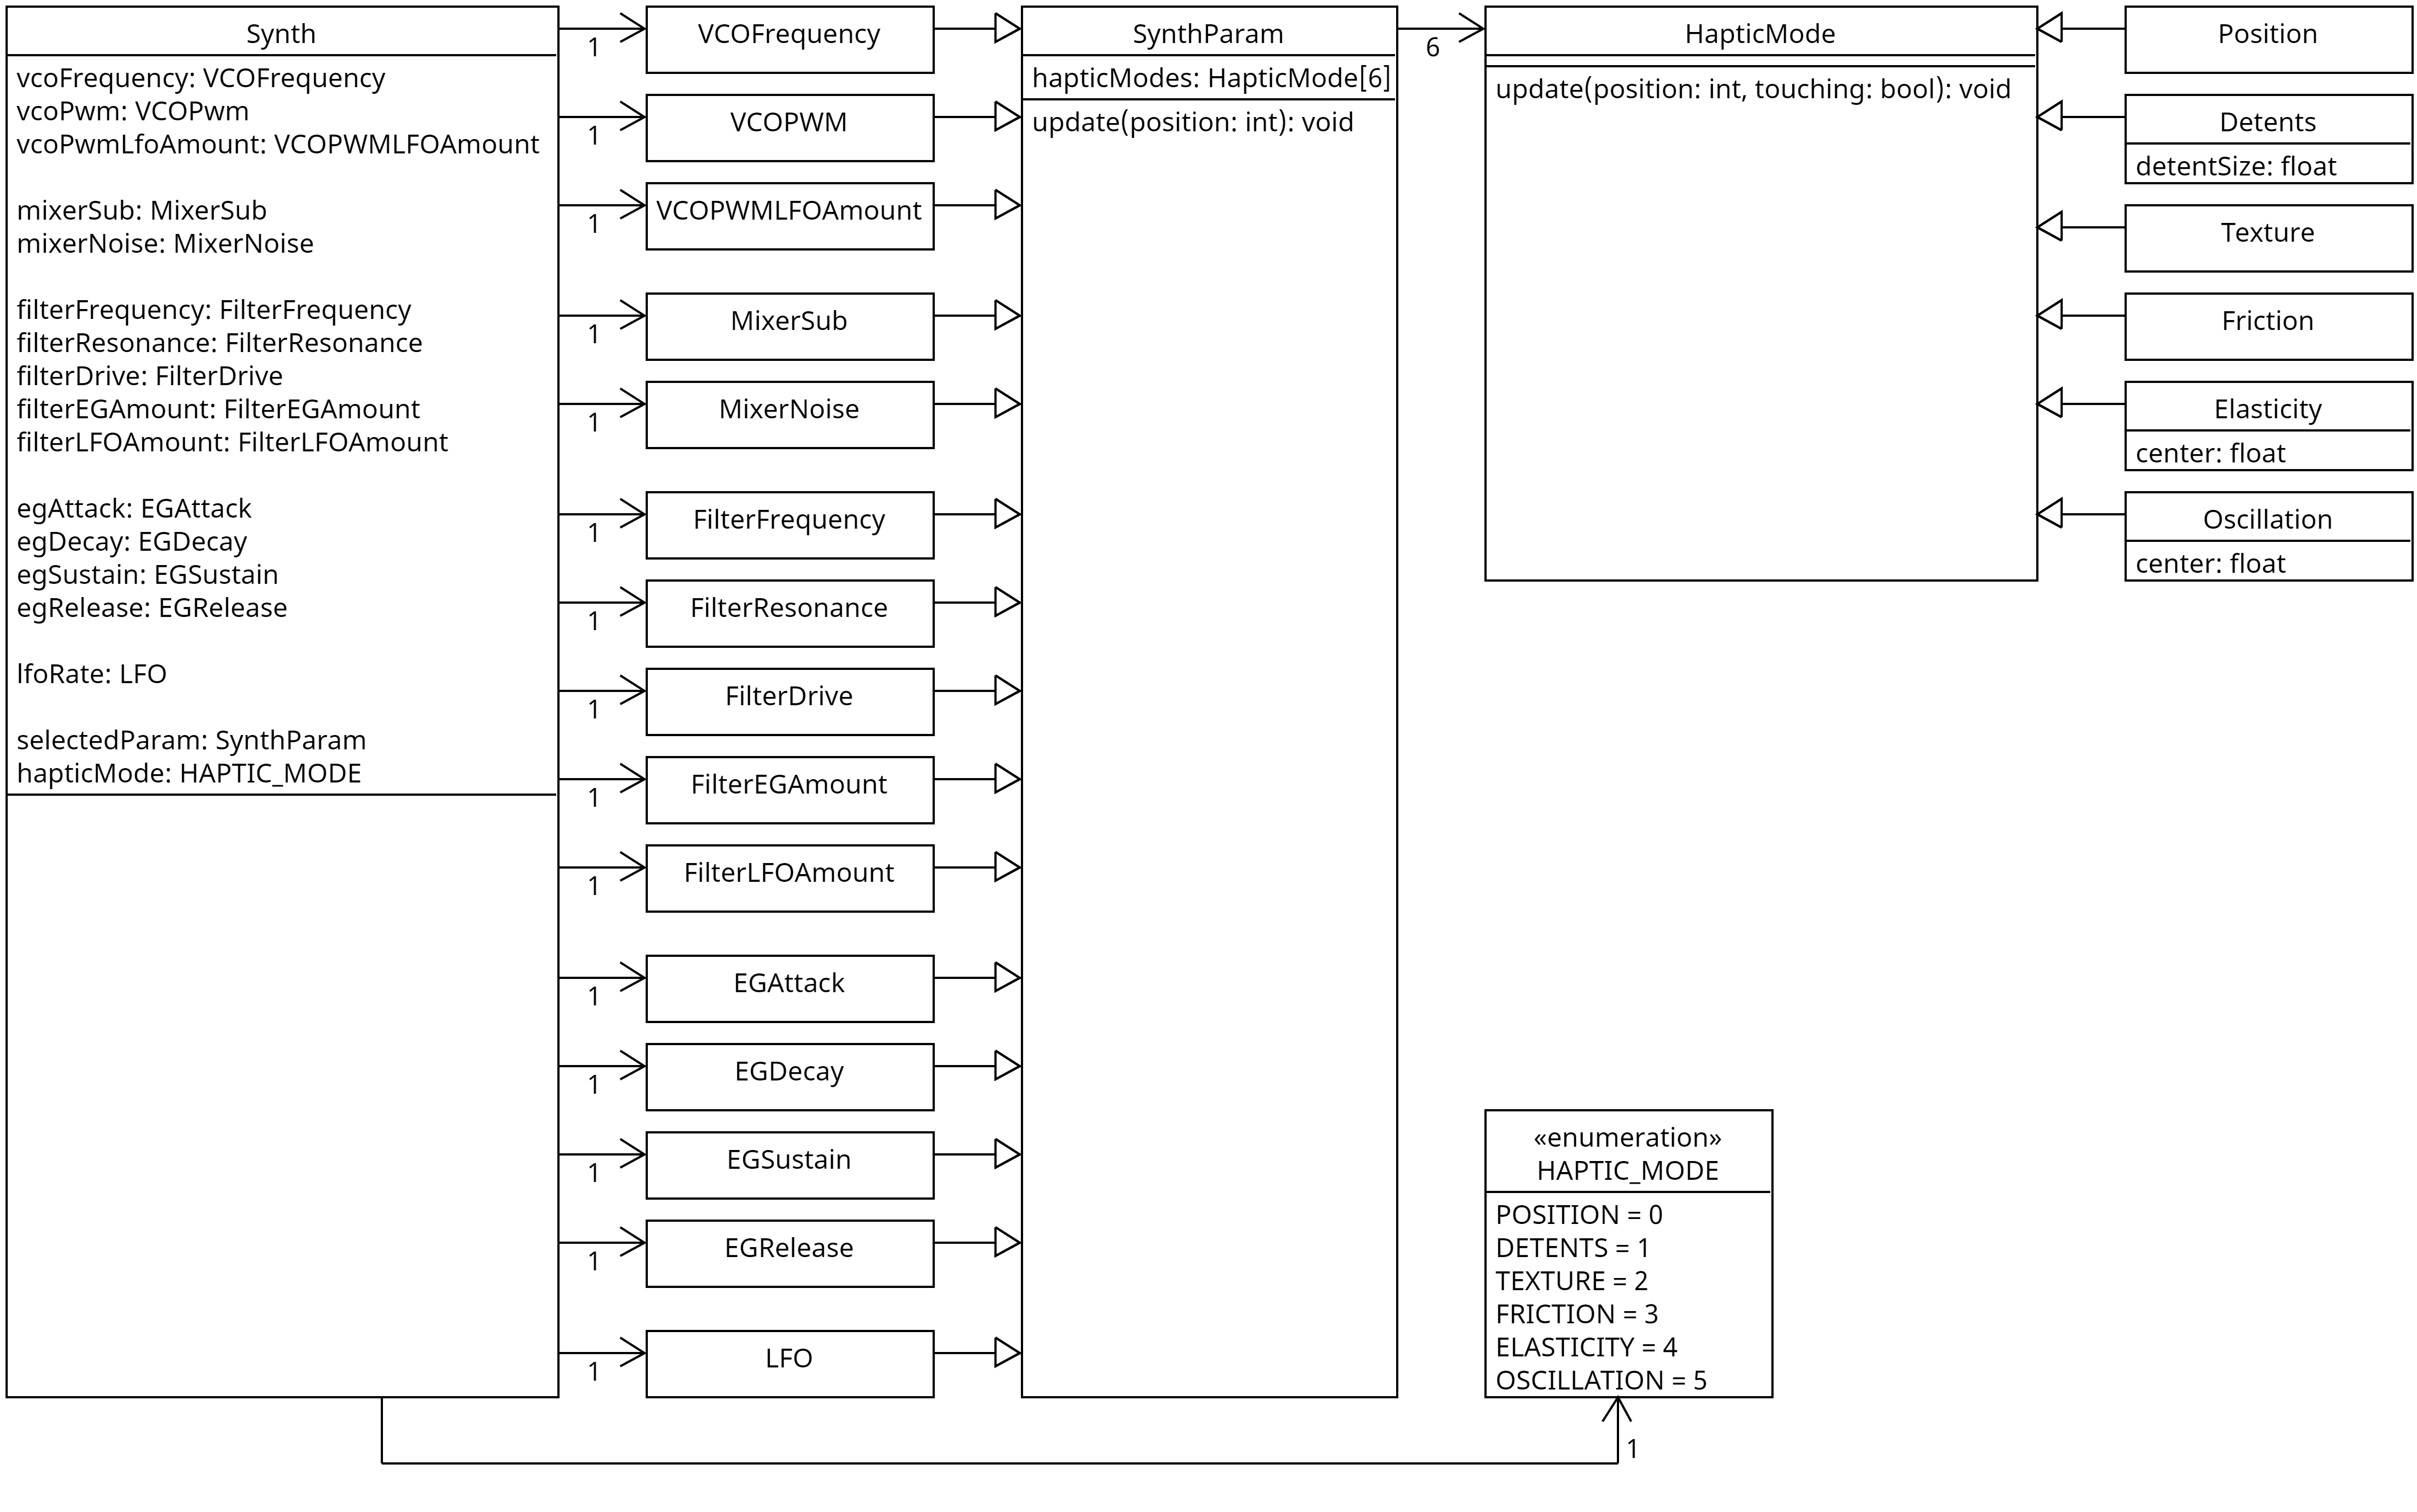
\includegraphics[width=1.0\linewidth]{figures/class-diagram.png}
	\caption{UML class diagram of HapSynth. \emph{\texttt{Synth}} has several \emph{\texttt{SynthParam}}s while each \emph{\texttt{SynthParam}} has one of each of the force feedback modes (\emph{\texttt{HapticMode}}). This way each synthesis parameter can have different response for each force feedback mode, i.e. different parameters can have different number of detents in Detents mode. \emph{\texttt{SynthParam}}'s \emph{\texttt{hapticModes}}-array is sorted so that the index of each force feedback mode matches respective values in \emph{\texttt{HAPTIC\_MODE}}.}
	\label{classdiagram}
\end{figure}

\section{User study} \label{userstudy}

The user study consisted of 15 participants. Participants were recruited from among the students of Haptic Interaction course in Tampere University and through word of mouth. Six participants had some prior experience using \glspl{dmi}, two had some knowledge of different sound synthesis methods, both being familiar with subtractive synthesis. Seven participants had used devices with force feedback. All participants chose to participate voluntarily and could withdraw from the study at any time without giving a reason. No personally identifying information was collected during the study. Before starting the studies, each participant filled an informed consent form agreeing to these terms.

As described earlier (see Chapter \ref{purpose}), user studies consisted of tasks using HapSynth, filling \gls{nasa-tlx} load questionnaires, and an interview. In addition, I conducted a brief preliminary information survey with each participant to examine their prior knowledge of \glspl{dmi}, sound synthesis and devices with force feedback. For participants who were not familiar with sound synthesis I briefly explained the basics of subtractive synthesis, and for all participants I showed how to operate HapSynth and encouraged them to try it out on their own to get necessary understanding of its working before beginning the tasks.

User study setup consisted of HapSynth, commercially available 37-key piano keyboard with built-in speakers, a laptop, and an audio interface. First twelve keys of the keyboard (keys $C1$--$B1$) were labelled with numbers 1-12, each key corresponding to one user task and its pre-recorded sound, while $C3$-key had its own indicator (see Figure \ref{keyboard}). \gls{midi} data from the keyboard was sent to the laptop running a \gls{daw} software that routed the first twelve keys of the keyboard to a software sampler and the rest to HapSynth, thus user could play pre-recorded samples with the first twelve keys and HapSynth using the rest. Audio from the laptop and HapSynth were mixed in an audio interface and routed to the internal speakers of the keyboard. In addition to the \gls{daw} software, the laptop also ran serial logger software to view and save the serial log from HapSynth. See Figure \ref{setup} for visual diagram of the setup. Along with the electronic devices a paper copy of Appendix \ref{ch:button} was provided for participants to reference the functions of the buttons.

\begin{figure}[h]
	\centering
	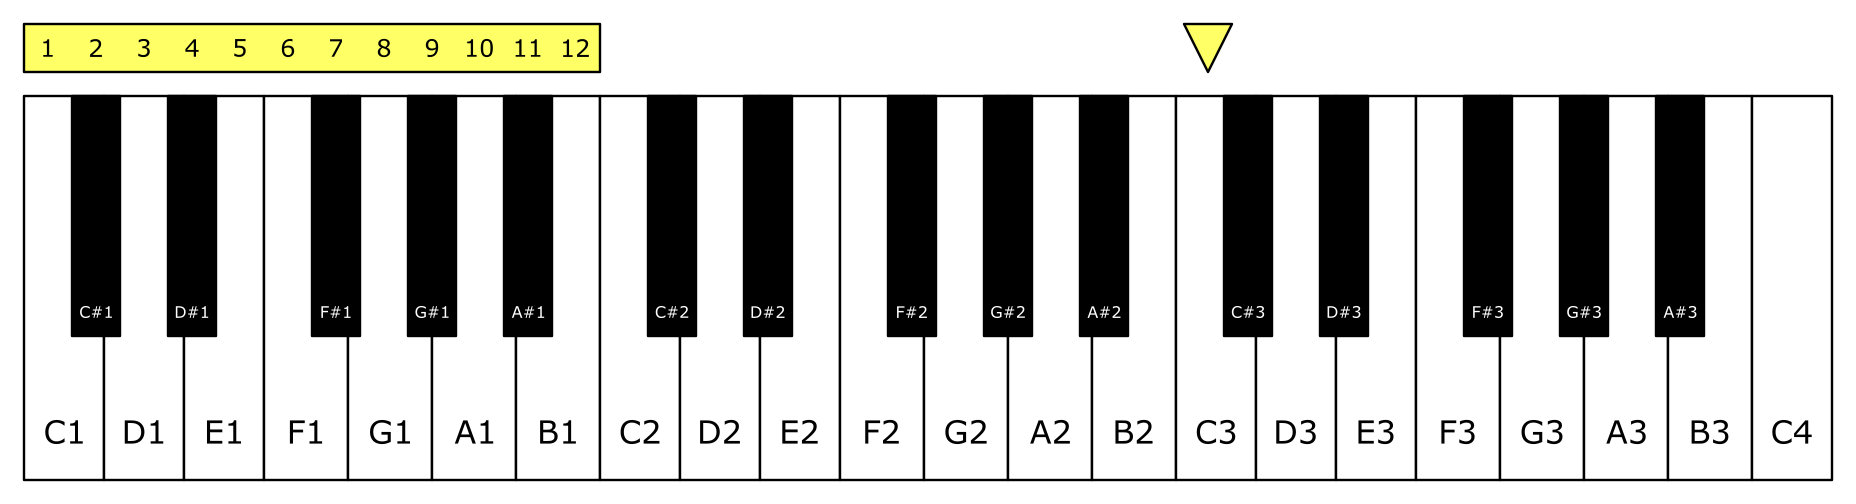
\includegraphics[width=1.0\linewidth]{figures/keyboard.png}
	\caption{Layout of the 37-key piano keyboard used in tests. Key names ($C1$, $C\#1$, $D1$ and so on) are overlayed on keys and yellow shapes on top of the keyboard represents the task/sound and $C3$-key labels.}
	\label{keyboard}
\end{figure}

\begin{figure}[h]
	\centering
	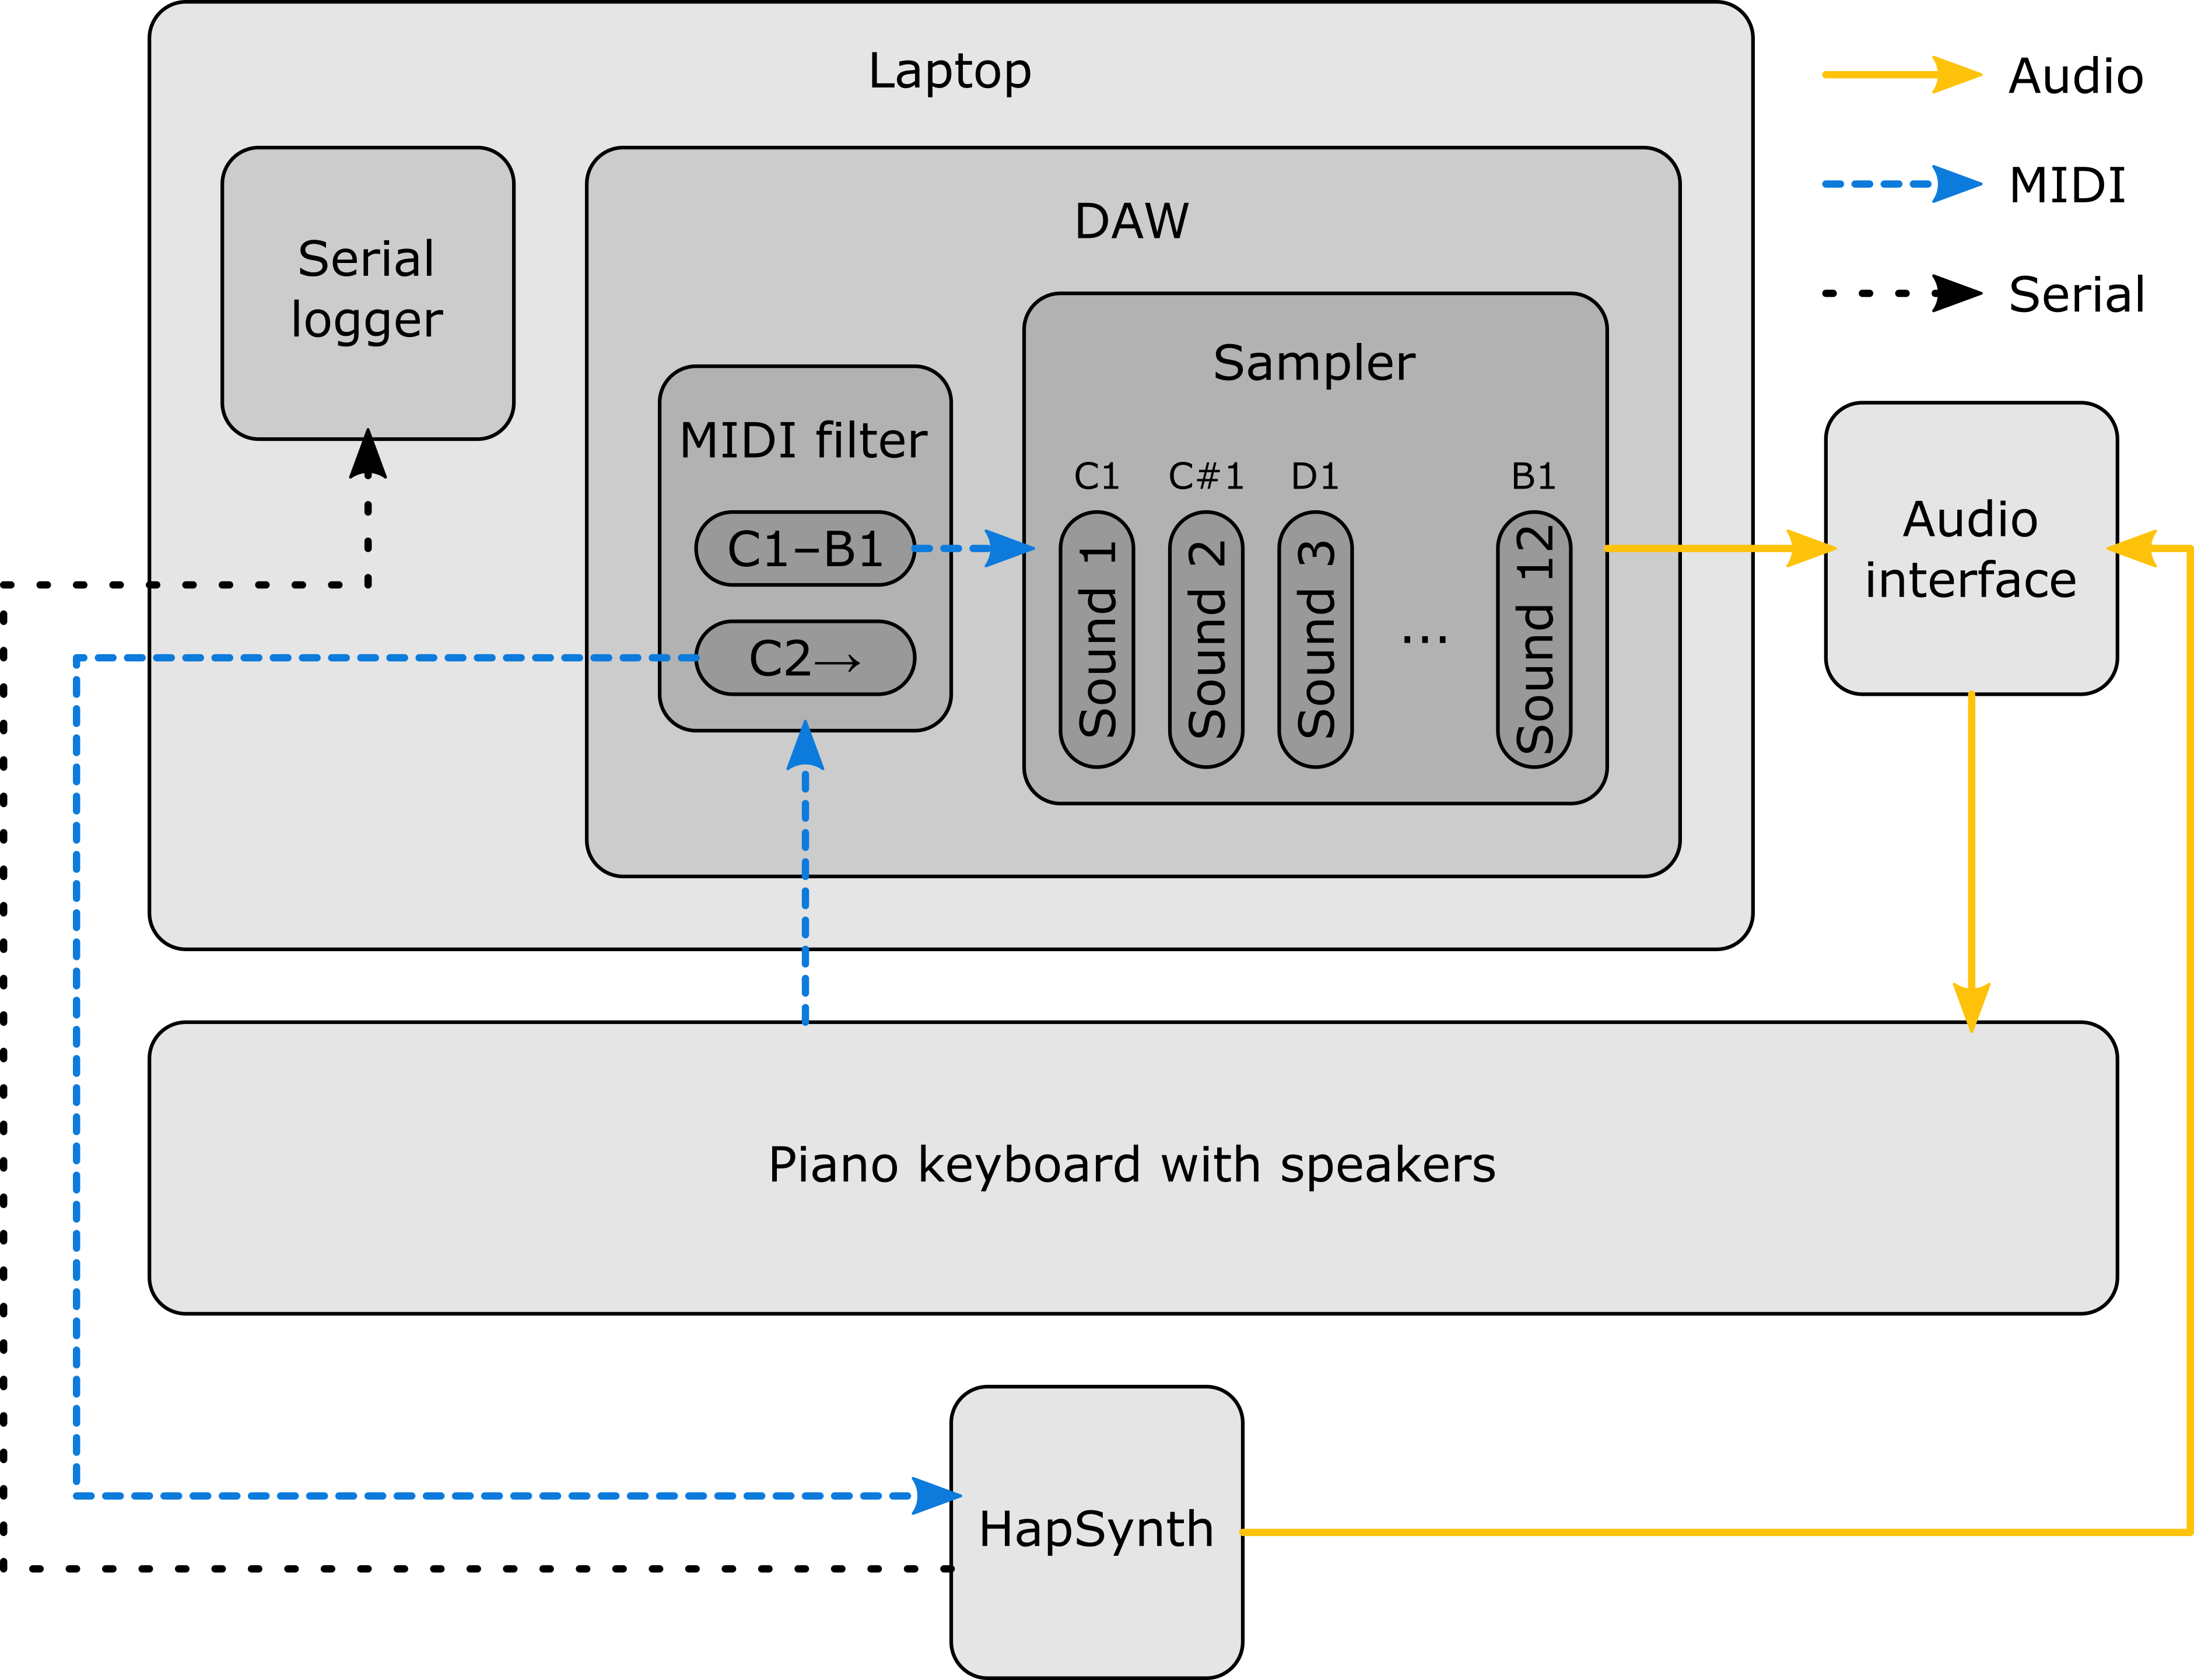
\includegraphics[width=1.0\linewidth]{figures/setup.png}
	\caption{Setup used in user tests. HapSynth is connected to the laptop with one \gls{usb} cable that relays both the \gls{midi} and serial data. Piano keyboard is connected to the laptop with a \gls{usb} cable. Audio interface is connected to the laptop with a \gls{usb} cable and to HapSynth and piano with audio cables.}
	\label{setup}
\end{figure}

Each participant had twelve tasks to complete. Tasks were grouped into four parts (indicated with letters $A$--$D$), where in each part a different force feedback mode was applied to the slider. Used force feedback modes were \textit{Detents}, \textit{Texture}, \textit{Friction}, and to draw comparison to \glspl{dmi} without force feedback, \textit{Position}. To counter learnability, different modes were applied to different parts for each participant, thus each participant experienced the modes in different order. \textit{Elasticity} and \textit{Oscillation} modes were left out from these tasks, as they don't allow leaving the slider to a set value, thus being unsuitable for the tasks.

Each task asked participants to change one or two given synthesis parameter values by moving the slider until the sound generated by HapSynth audibly matched to a pre-recorded sample. Each sample was recorded by setting HapSynth's parameters to the target value of a task programmatically and playing $C3$-key. Participants could listen to the pre-recorded sound by playing a key of the keyboard that was labelled with the task's number, and HapSynth by playing $C3$-key (or any un-labelled key, though $C3$-key is the one used for comparisons since that matches the pitch of the samples). Each part had three tasks with the following assignments always in the same order (so tasks 1, 4, 7, and 10 each had assignment 1, tasks 2, 5, 8, and 11 assignment 2 and so on):

\begin{enumerate}
	\item Change filter's cutoff frequency to match recorded sound
	\item Change envelope generator's attack time to match recorded sound
	\item Change LFO's frequency and oscillator's LFO amount to pulse width modulation to match recorded sound
\end{enumerate}

Table \ref{targets} shows the target value for each task. Value of 0 represents the slider in its left most position while 100 represents the right most position. With detents mode values 25 and 75 were one of the detents for each parameter (very easy to get exactly the right value), while 40 and 60 were not (impossible to get the right value). Values for tasks were designed so that no matter the order of the force feedback modes, in detents mode each participant would be able to get two values exactly right and two values would be impossible to get right. This allowed me to observe both the advantage and disadvantage that detent mode inherently causes and see whether those affected the participants' satisfaction and frustration, respectively.

\begin{table}[h!]
	\centering
	\begin{tabular}{|c||c|c||c|c|c|c|}
		\hline
		\multirow{3}{*}{\thead{Task}} & \multirow{3}{*}{\thead{Part}} & \multirow{3}{*}{\thead{\begin{tabular}[c]{@{}c@{}}Assign- \\ ment\end{tabular}}} & \multicolumn{4}{c|}{\thead{Target value (0-100)}} \\\cline{4-7}
			&&& \thead{Filter cutoff} & \thead{EG attack} & \thead{LFO fre-} & \thead{Oscillator LFO} \\
			&&& \thead{frequency} & \thead{time} & \thead{quency} & \thead{amount to PWM} \\
		\hline
		\hline
			1 & \multirow{3}{*}{$A$} & 1 & 60 & x & x & x \\ \cline{1-1} \cline{3-7}
			2 &                      & 2 & x & 25 & x & x \\ \cline{1-1} \cline{3-7}
			3 &                      & 3 & x & x & 40 & 75 \\
		\hline
		\hline
			4 & \multirow{3}{*}{$B$} & 1 & 40 & x & x & x \\ \cline{1-1} \cline{3-7}
			5 &                      & 2 & x & 60 & x & x \\ \cline{1-1} \cline{3-7}
			6 &                      & 3 & x & x & 75 & 25 \\
		\hline
		\hline
			7 & \multirow{3}{*}{$C$} & 1 & 25 & x & x & x \\ \cline{1-1} \cline{3-7}
			8 &                      & 2 & x & 75 & x & x \\ \cline{1-1} \cline{3-7}
			9 &                      & 3 & x & x & 60 & 40 \\
		\hline
		\hline
			10 & \multirow{3}{*}{$D$} & 1 & 75 & x & x & x \\ \cline{1-1} \cline{3-7}
			11 &                      & 2 & x & 40 & x & x \\ \cline{1-1} \cline{3-7}
			12 &                      & 3 & x & x & 25 & 60 \\
		\hline
	\end{tabular}
	\caption{Parts, assignments, and target synthesis parameter values for different tasks.}
	\label{targets}
\end{table}

When a participant thought they were as close to the target value as possible, they would announce that out loud. I measured the time the participant took in seconds and the distance(s) to the target value(s) in the units described above. These measurements were recorded for later analysis and not shown to the participant. If a participant took long time in one task, I asked them to stop and move to the next task. Results of these halted tasks were not included in the data analysis.

After each part I asked participants to fill out a \gls{nasa-tlx} load questionnaire to measure their perceived workload of the used force feedback mode. \gls{nasa-tlx} is developed by NASA in 1986 to evaluate workload using six dimensions: \textit{mental demand}, \textit{physical demand}, \textit{temporal demand}, \textit{own performance}, \textit{effort}, and \textit{frustration} (\cite{hart1986}). First, participants weight the relative importance of each dimension using pair-wise comparisons between them, and then they rate each dimension in a scale from 0 to 100 (higher number corresponding to higher workload). Finally, a weighted average is taken from the ratings giving the total score. (\cite{hart1986}). To shorten the duration of the user studies, I opted to utilize Raw TLX variation of \gls{nasa-tlx} which omits the weighting procedure of the dimensions (\cite{hart2006}). Omitting weighting has been shown both increasing and decreasing the sensitivity of the measurements, thus both methods seem equally valid (\cite{hart2006}).

Finally, after all the tests, I conducted a short interview. The interviews were semi-structured with open questions exploring the topics of overall experience using HapSynth, pros and cons of each individual mode, and benefits/drawbacks of having force feedback in a \gls{dmi} in general. Semi-structured interviews allow to focus into the topics that interest the participants and skip those that do not (\cite{lazar2017}), and with them I could gather more data with the limited sample size, thus I chose them for this study.

Along with the interviews I allowed the participants to freely use HapSynth to remind themselves how each of the force feedback modes felt. I also encouraged them to try out \textit{Elasticity} and \textit{Oscillation} modes, as they weren't part of the user tasks, but I was still interested to learn what the participants thought of them.

\section{Analysis methods}

User studies were analysed with qualitative and qualitative analysis methods. Interviews were analysed with thematic analysis using emergent coding, while one-way \glspl{anova} and pairwise comparisons were conducted for the \gls{nasa-tlx} and measured data from the tasks.

\textit{Qualitative data.} Thematic analysis using emergent coding was chosen for the analysis method of the interview data. Previous literature is relatively sparse on specifically \glspl{dmi} with force feedback, hence emergent coding was more appropriate method than priori coding (\cite{lazar2017}).

During the interviews participants' key observations were noted down, and later from the notes of all interviews repeating phenomena were identified and grouped into codes, such us "Force feedback assures user that the device is working" and "Too strong feedback can be unpleasant". These codes were grouped into concepts (i.e. "Force feedback helps user" and "Force feedback is unpleasant and hinders performance"), which were further grouped into categories ("Varying opinions on enjoyability and usefulness").

\textit{Quantitative data.} \gls{nasa-tlx} and measured data were analysed with statistical methods. For both one-way \gls{anova} tests were conducted with force feedback modes as independent variables. If some statistical significance was found from those, pairwise comparisons were used to further investigate the difference between the modes.